% This must be in the first 5 lines to tell arXiv to use pdfLaTeX, which is strongly recommended.
\pdfoutput=1
\documentclass[11pt]{article}

% Change "review" to "final" to generate the final (sometimes called camera-ready) version.
% Change to "preprint" to generate a non-anonymous version with page numbers.
% \usepackage[review]{acl}
% \usepackage[final]{acl}
\usepackage[preprint]{acl}

% This assumes your files are encoded as UTF8
\usepackage[utf8]{inputenc}

% Standard package includes
\usepackage{times}
\usepackage{latexsym}

% For proper rendering and hyphenation of words containing Latin characters (including in bib files)
\usepackage[T1]{fontenc}

% This is not strictly necessary, and may be commented out,
% but it will improve the layout of the manuscript,
% and will typically save some space.
\usepackage{microtype}

% This is also not strictly necessary, and may be commented out.
% However, it will improve the aesthetics of text in
% the typewriter font.
\usepackage{inconsolata}

%Including images in your LaTeX document requires adding
%additional package(s)
\usepackage{graphicx}
% \usepackage{arydshln}
\usepackage{tabularx}
\usepackage{multirow}
\usepackage{booktabs}
\usepackage{tcolorbox}
\usepackage{listings}
\usepackage{soul}

\lstnewenvironment{prompt}[1]
{%
    \lstset{
      caption=#1,
      captionpos=b,
      basicstyle=\ttfamily\small,
      columns=fullflexible,
      frame=single,
      breaklines=true,
      breakindent=0pt,
      backgroundcolor=\color{gray!10}
    }%
}{}

\renewcommand\lstlistingname{Prompt}
\renewcommand\lstlistlistingname{Prompt}

% Better URL line breaks in References
\def\UrlBreaks{\do\/\do-}

\usepackage{xcolor}

\usepackage{xspace}
\newcommand{\DCLM}{\textsc{DCLM}\xspace}
%\newcommand{\Ours}{Ours\xspace} % ANON - uncomment this
\newcommand{\Ours}{Nemotron-CC\xspace}

% ANON - remove Nemotron-CC from title
\title{Nemotron-CC: Transforming Common Crawl into a Refined Long-Horizon Pretraining Dataset}

\author{
 \textbf{Dan Su\textsuperscript{*}},
 \textbf{Kezhi Kong\textsuperscript{*}},
 \textbf{Ying Lin\textsuperscript{*}},
 \textbf{Joseph Jennings},
 \textbf{Brandon Norick},
\\
 \textbf{Markus Kliegl\textsuperscript{\textdagger}},
 \textbf{Mostofa Patwary},
 \textbf{Mohammad Shoeybi},
 \textbf{Bryan Catanzaro}
\\
\\
  NVIDIA
\\
 \small{
   \textsuperscript{*}Equal contribution. \textsuperscript{\textdagger}Correspondence to \href{mailto:mkliegl@nvidia.com}{mkliegl@nvidia.com}.
 }
}

\begin{document}
\maketitle
\begin{abstract}
Recent English Common Crawl datasets like FineWeb-Edu and \DCLM achieved significant benchmark gains via aggressive model-based filtering, but at the cost of removing $90\%$ of data. This limits their suitability for long token horizon training, such as 15T tokens for Llama 3.1. In this paper, we show how to achieve better trade-offs between accuracy and data quantity by a combination of classifier ensembling, synthetic data rephrasing, and reduced reliance on heuristic filters.
When training 8B parameter models for 1T tokens, using a high-quality subset of our data improves MMLU by 5.6 over \DCLM, demonstrating the efficacy of our methods for boosting accuracies over a relatively short token horizon. Furthermore, our full 6.3T token dataset matches \DCLM on MMLU, but contains four times more unique real tokens than \DCLM. This unlocks state-of-the-art training over a long token horizon: an 8B parameter model trained for 15T tokens, of which 7.2T came from our dataset, is better than the Llama 3.1 8B model: +5 on MMLU, +3.1 on ARC-Challenge, and +0.5 on average across ten diverse tasks.
% ANON - Remove or edit sentence below.
The dataset is available at \url{https://data.commoncrawl.org/contrib/Nemotron/Nemotron-CC/index.html}.
\end{abstract}

\section{Introduction}

\begin{figure}[th!]
\centering
% ANON - change figure
% \includegraphics[width=\linewidth]{figures/figure1anon.pdf}
% \\\vspace{-2\belowdisplayskip}
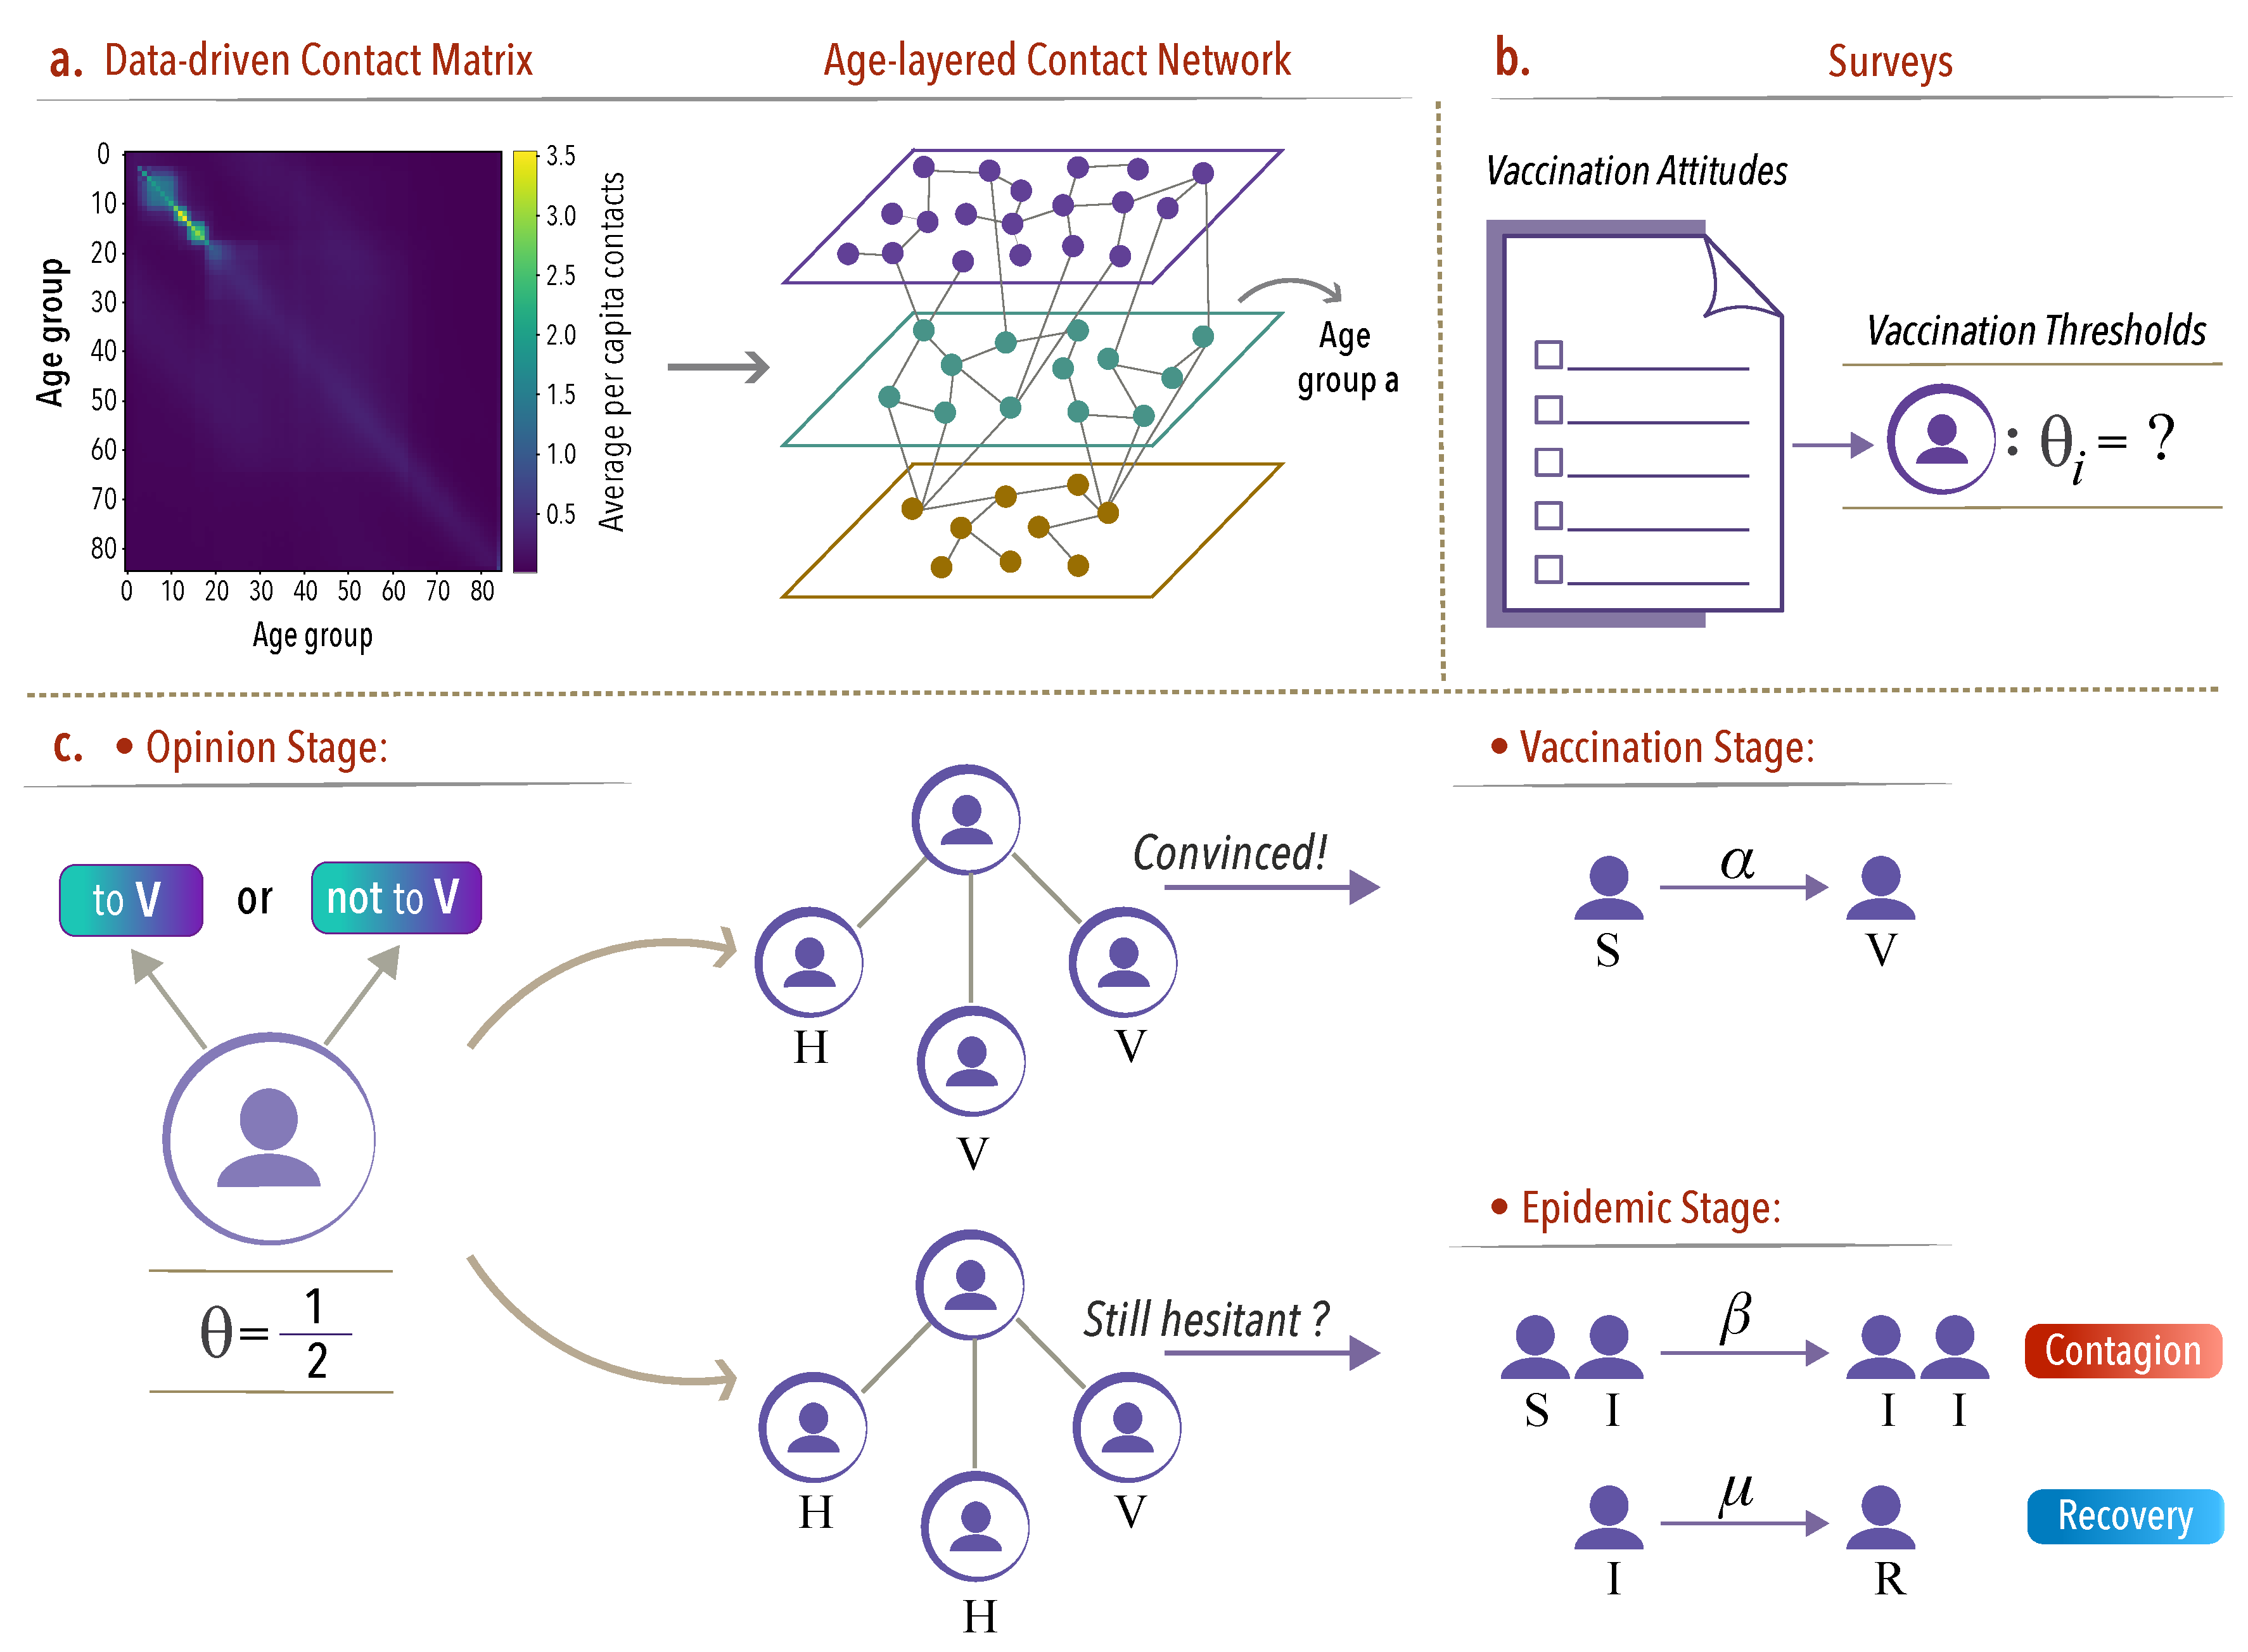
\includegraphics[width=0.8\linewidth]{figures/figure1.pdf}
\caption{MMLU scores for 8B parameter models trained for 1T tokens. Compared to \DCLM, our methods enable us to either create a 4$\times$ larger dataset of similar quality or increase the MMLU using a high quality subset of the tokens. Having a larger dataset, in the sense of unique real tokens, is crucial when training over long horizons such as 15T tokens.}
\label{fig:main}
\end{figure}

Internet crawl is the largest source of unique tokens for training LLMs and can be seen as serving two main purposes: high-quality content and diversity.  Recent English datasets derived from Common Crawl\footnote{\url{https://commoncrawl.org/}} such as FineWeb-Edu~\citep{penedo2024fineweb} and \DCLM~\citep{li2024datacomp} have emphasized high-quality content that boosts benchmark accuracies over data quantity. They have demonstrated significant strides in achieving benchmark results competitive with some of the best closed models at a small scale (e.g., DCLM's 7B model trained over 2.6T tokens), primarily thanks to the use of model-based filters to extract high-quality educational and instructional content. However, this comes at the cost of data quantity: they remove around $90\%$ of the data.
Such aggressive pruning may not be the most effective strategy when training larger models over longer token horizons (e.g., Llama 3.1 includes 8B--405B parameter models, trained for 15T tokens~\citep{dubey2024llama} and Gemma 2 27B was trained for 13T tokens~\citep{team2024gemma}).
Both \DCLM and FineWeb-Edu contain around $80\%$ near-duplicates (1T and 0.2T unique tokens, respectively)~\citep{fineweb-edu-discussion,li2024datacomp} and to train on these datasets for many trillions of tokens implies seeing essentially the same samples many times during training. This could lead to inferior models, as \citet{muennighoff2024scaling} find there are diminishing returns after four epochs compared to training on more unique tokens.

In this paper, we show how to achieve a better trade-off between benchmark accuracy and data quantity with a combination of classifier ensembling, synthetic data generation, and reduced reliance on heuristic filters. Our main contributions are:
\begin{enumerate}
\item We propose a method for transforming English Common Crawl into a 6.3T token long-horizon pretraining dataset, consisting of 4.4T globally deduplicated original tokens and 1.9T synthetically generated tokens.
% ANON - Remove sentence below
We release the dataset\footnote{\url{https://data.commoncrawl.org/contrib/Nemotron/Nemotron-CC/index.html}} and plan to release an implementation as part of the open-source NeMo Curator library.\footnote{\url{https://github.com/NVIDIA/NeMo-Curator}}
\item We prove the effectiveness of this method by comparing to the state-of-the-art open English Common Crawl datasets \DCLM and FineWeb-Edu~(Figure~\ref{fig:main}).
\begin{enumerate}
\item A 1.1T-token high-quality subset of our data achieves a 5.6 MMLU improvement over \DCLM, showing the superiority of our method over a relatively short token horizon.
\item Our full dataset performs on par with \DCLM while having 4$\times$ as many unique real tokens.
\item This larger size enables state-of-the-art results over long token horizons: An 8B parameter model trained for 15T tokens using a weighted version of our dataset achieves higher overall accuracy than Llama 3.1 8B, and in particular MMLU 70.3 vs. Llama's 65.3. Note that Llama 3.1 8B was also trained on 15T tokens~\citep{dubey2024llama}.
\end{enumerate}
\item We conduct ablation studies and find:
\begin{enumerate}
\item Ensembling different model-based classifiers can help select a larger and more diverse set of high quality tokens.
\item Rephrasing can effectively reduce noise and errors in low-quality data and produce diverse variants with fresh unique tokens from high-quality data, leading to better results in downstream tasks.
\item Disabling traditional non-learned heuristic filters for high-quality data can further boost high quality token yield without hurting accuracy.
\end{enumerate}
\end{enumerate}

Finally, we remark that our overall guiding principle is to shift from a static, non-learned, heuristic pipeline towards a more learned flywheel whose performance will naturally get better over time. As our data improves, so will the LLMs we train, and these improved LLMs will in turn improve our data as we use them to generate better synthetic data and quality classifications.

\section{Methods}

In this section we explain our efforts to build the best English Common Crawl pretraining dataset for LLMs. Our efforts can be splitted into three folds. First, we talk about our efforts in boosting token yield by utilizing text extractor and heuristic filters more properly in Section~\ref{sec:extract_filter}. Second, we introduce the model-based quality labeling pipeline methods in Section~\ref{sec:classifier}. Third, we introduce our synthetic data generation method to further improve the data quality in Section~\ref{sec:synthetic}.

\subsection{HTML-to-text Extractor \& Filter} \label{sec:extract_filter}
Extracted texts from HTMLs are the foundation and major source of LLM pretraining dataset, so it is of great significance to analyze and understand the extraction tools for optimal data quality and token yield. Moreover, heuristic filters are often utilized to remove low-quality tokens with human-designed heuristics \citep{li2024datacomp,parmar2024data,penedo2024fineweb,dubey2024llama}, which may also put good tokens at the risk of being removed. We carefully examine both aspects with the assist of the FineWeb-Edu classifier \citep{penedo2024fineweb}, a model-based quality classifier that had shown effectiveness in identifying high-quality tokens that are significant in boosting the strength of LLMs.

\begin{table}[htbp] \small \centering
\begin{tabular}{@{}lccc@{}}
\toprule  
                     & \textbf{\#Tokens} & \textbf{\#HQ tokens} & \textbf{\#HQ +\%} \\ \midrule
Trafilatura-filtered & 994              & 80                  & -                       \\
Justext-filtered     & 1,380            & 104                 & 28.6\%                  \\
Justext              & 1,804            & 127                 & 57.4\%                  \\ \bottomrule
\end{tabular}
\caption{Extraction and filteration token count statistics (billion). Tokens counted after deduplication.}
\label{table:extract_filter_stats}
\end{table}

% The tabularx version has a linebreak in Trafilatura-\nfiltered - doesn't look good
% \begin{table}[htbp] \small \centering
% \begin{tabularx}{\linewidth}{Xccc}
% \toprule  
%                      & \textbf{\#Token} & \textbf{\#HQ token} & \textbf{\#HQ +\%} \\ \midrule
% Trafilatura-filtered & 994              & 80                  & -                       \\
% Justext-filtered     & 1,380            & 104                 & 28.6\%                  \\
% Justext              & 1,804            & 127                 & 57.4\%                  \\ \bottomrule
% \end{tabularx}
% \caption{Extraction and filteration token count statistics (billion). Tokens counted after deduplication.}
% \label{table:extract_filter_stats}
% \end{table}

\paragraph{HTML-to-text Extraction} We test two HTML-to-text extractors, Justext~\citep{pomikalek2011removing} and Trafilatura~\citep{barbaresi-2021-trafilatura}. Qualitatively, we view both extractors at the same level of quality. While quantitatively, we calculate token yields of both extractors on 13 selected snapshots of Common Crawl (see Appendix~\ref{sec:13_snapshots}). The statistics were reported in Table~\ref{table:extract_filter_stats}. We see that Justext can yield more tokens, notably more high-quality tokens (+28.6\%) by the standard of Fineweb-Edu classifier (score 3, 4, and 5). We highlight that, boosting unique token amount is of great importance when building long-horizon pretraining dataset, e.g., 15T tokens for Llama3.1.
We keep only English text, as determined by pycld2\footnote{\url{https://pypi.org/project/pycld2/}} and the FastText lid176 language classifier\footnote{\url{https://fasttext.cc/docs/en/language-identification.html}} with threshold 0.3~\citep{joulin2016fasttext,joulin2016bag}.
After extraction, we apply global fuzzy deduplication as well as exact substring deduplication~\citep{lee2022deduplicating}, using the NeMo Curator library\footnote{\url{https://github.com/NVIDIA/NeMo-Curator}} and the deduplicate-text-datasets library,\footnote{\url{https://github.com/google-research/deduplicate-text-datasets}} respectively.

\paragraph{Filtering} Conventionally, heuristic filters are leveraged to remove low-quality tokens from the pretraining dataset as a post-processing step \citep{li2024datacomp,parmar2024data,penedo2024fineweb,dubey2024llama}. We revisit the filtering pipeline as in \citep{parmar2024data}. Such pipeline sequentially consists of a set of heuristic filters proposed by \citet{raffel2020exploring,rae2021scaling} and a perplexity filter based on a KenLM model~\citep{heafield2011kenlm} trained on Wikipedia and books data~\citep{wenzek-etal-2020-ccnet}. To quantitatively better understand the effectiveness of the filtering pipeline, we calculate the token yield and report the numbers in Table \ref{table:extract_filter_stats}. We find the filtering pipeline removes a non-trivial portion of high-quality tokens (-18.1\%) classified by FineWeb-Edu classifier from the dataset. 

Given the impact that the heuristic filters have on the high-quality token yield, we propose to NOT apply such filters to the high-quality tokens distinguished by model-based quality classifers (described in the next section), but only use those on the low-quality splits. In the experiment section we empirically verify the impact of both the extractor and filter on pretraining data quality through downstream benchmarks. We refer readers to Section~\ref{sec:ablation} for detailed results.

\subsection{Model-based Quality Labeling} \label{sec:classifier}
Recent work~\citep{li2024datacomp,penedo2024fineweb} use model-based classifiers to extract high-quality pretraining documents from English Common Crawl. However, both of the two quality classifiers have a limited recall (less than 10\%) of high-quality tokens, and this will become a bottleneck to train an LLM over a long horizon. Also, the quality labels assigned by the quality classifier are not necessarily aligned with LLM's downstream task performance. Therefore, we propose our ensemble-based quality labeling pipeline method. Specifically, we first build three quality classifiers, each of which has different high-quality preferences. Then, we ensemble the three classifiers to score all the documents, and split the crawl corpus into different quality buckets based on the quality score. Finally, we regroup the fine-grained document buckets into 5 different quality levels based on their corresponding performance on downstream task. 

\paragraph{Quality Classifier Training}
Preparing pretraining documents with quality annotations is the first key step in building a quality classifier~\citep{dubey2024llama,abdin2024phi,yang2024qwen2}. Similar to the work ~\citep{penedo2024fineweb}\footnote{We use the same 460K document samples as in the FineWeb-Edu-Annotation dataset.}, we constructed two versions of quality annotation data. We prompt Mistral 8x22B-instruct\footnote{\url{https://mistral.ai/news/mixtral-8x22b/}} and Nemotron-340B-instruct~\citep{adler2024nemotron}, to score web documents from FineWeb based on their educational value on a scale from 0 to 5.  We then fine-tune a linear regression model on top of the Snowflake-arctic-embed-m embedding model~\citep{merrick2024arctic} using the two different version of training sets. The two models have been trained for 20 epochs with a learning rate of 3e-4, with the embedding and encoder layers frozen, and we selected the checkpoint with the highest F1 score on
the held-out validation set.

 We also employ the DCLM classifier which is a fastText-based classifier released by~\citet{li2024datacomp}. The DCLM classifier is trained on a combination of instruction-formatted data~\citep{OpenHermes} and high-scoring posts data from ELI5 subreddit~\citep{fan2019eli5}, and has shown stronger performance in identifying high-quality pretraining tokens, compared to the FineWeb-Edu classifier ~\citep{penedo2024fineweb}. The DCLM classifier will offer a new perspective in labeling high-quality pretraining documents, and will help increase the recall of high-quality tokens.

\paragraph{Quality Scoring and Bucketing}
First, we use each of the three classifiers to predict the quality scores for all the documents. Then based on the ranked quality score from each classifier, we rounded the model's output score to integers from 0 to 19. So that each score bucket will have around 5\% of the documents, and bucket 19 will have the top 5\% highest quality documents. We then assign the final quality score for each document by ensembling the three classifiers' integer score by a maximum operation. The number of documents distribution in each buckets will be skewed by the ensemble operation.

\paragraph{Quality Labeling}
In order to assign a quality label that is more aligned with their real performance on downstream tasks, we further group the fine-grained quality score predicted by three classifiers into 5 downstream quality categories. We used annealing to access each data bucket's downstream task's quality. Specifically, we measure the quality of each bucket by continuous pretraining with 50B tokens on a 70\% trained 8B models. We assign 66\% of weight to the default data mix and 34\% to the dataset that we are evaluating. By comparing the average performance of each bucket over 9 tasks, we group the 20 buckets into 5 big categories, with the final distribution shown in Table~\ref{table:quality_label_stats}.

\begin{table}[htbp]\centering\small
\begin{tabularx}{\linewidth}{Xcc}
\toprule
\textbf{Quality Label} & \multicolumn{1}{l}{\textbf{Buckets}} & \multicolumn{1}{l}{\textbf{Token ($\%$)}}  \\ \midrule
High                   & 19                                    & 12.63                                       \\
Medium-High            & 18                                    & 11.52                                       \\
Medium                 & 12-17                                 & 46.24                                       \\
Medium-Low             & 7-11                                  & 20.43                                       \\
Low                    & 0-6                                   & 9.18                                        \\ \bottomrule
\end{tabularx}
\caption{Common Crawl quality labels statistics.}
\label{table:quality_label_stats}
\end{table}

\subsection{Synthetic Data Generation} \label{sec:synthetic}

Upon reviewing samples across the quality tiers, we observe that documents with lower scores tend to contain more noise and errors, while those scoring higher generally exhibit good writing and formatting.
Therefore, we employ different strategies when generating data from low- and high-quality documents.

For low-quality data, our goal is to improve the quality by reducing noise and errors while preserving useful information, thereby decreasing training compute expenses. As shown by~\citet{maini2024rephrasing}, rephrasing web data using a medium-sized language model yields an enhanced parallel corpus of synthetic data, thereby reducing model perplexity and boosting its accuracy on downstream tasks.
Unlike existing methods that create new content such as textbooks and short stories~\cite{wang2023self,eldan2023tinystories,gunasekar2023textbooks}, our rephrasing-based approach does not utilize the language model as a knowledge bank but focuses on transforming provided texts into another style, allowing it to operate with a lighter-weight model.
We adopt the \textrm{Wikipedia} style prompt from~\citep{maini2024rephrasing}
% (i.e., ``\textit{For the following paragraph give me a diverse paraphrase of the same in high quality English language as in sentences on Wikipedia}'')
to rewrite low-quality documents (Prompt~5 in Appendix~\ref{sec:appendix-prompt-templates}), which effectively reduces errors and redundancies and improves formatting.

For high-quality data, we aim to obtain more unique tokens and condense essential knowledge. According to~\citep{muennighoff2024scaling}, adding repeated tokens yields a diminishing return, especially after 4 epochs.
For high-quality documents, we generate synthetic data using four additional prompts:
(1) \textrm{Diverse Question-Answer (QA) pairs}: ask questions in various forms (e.g., yes/no question, open-ended question, multi-choice question) about factual information in the text and provide the correct answers;
(2) \textrm{Distill}: rewrite the text into a concise and clear passage;
(3) \textrm{Extract knowledge}: rewrite knowledge from the text and disregard uninformative content;
(4) \textrm{Knowledge list}: extract key information from the text as an organized list.
We require the model to provide clear and concise responses while preserving factual information and concrete details such as numbers.
The full prompts are shown in Appendix~\ref{sec:appendix-prompt-templates}.

As we increase the length of provided text, the model shows a tendency to produce over-simplified outputs with reduced detail. Therefore, we chunk each document into segments, each of which contains one or more complete lines and is shorter than a specific token limit.\footnote{The token limit is set to 512 for \textrm{Wikiepdia}, 2,000 for \textrm{Distill}, 1,400 for \textrm{Extract Knowledge} and 1,000 for \textrm{Diverse QA Pairs} and \textrm{Knowledge List}, including tokens from the prompt and chat format.} Over-length lines exceeding the token limit are discarded.

\begin{tcolorbox}[boxsep=0mm,left=1mm,right=1mm,top=1mm,bottom=1mm,fontupper=\small\ttfamily,halign=left,arc=0mm,boxrule=1pt,colback=gray!10]
\textbf{Question}: Which year did the United Nations implement the 2030 agenda for SDGs?

\textbf{Answer}: January 1, 2016

\vspace{4pt}

\textbf{Question}: What are the three key dimensions of sustainable development covered by the SDGs?

\textbf{Answer}: (a) economic growth, (b) social inclusion, and (c) environmental protection

\vspace{4pt}

\textbf{Question}: Which of the following can flossing prevent? A) Cavities B) Gum disease C) Both A and B D) Neither A nor B

\textbf{Answer}: C) Both A and B

\vspace{4pt}

\textbf{Question}: Is flossing important even if you brush your teeth twice a day?

\textbf{Answer}: Yes, flossing is important as it reaches areas that brushing alone cannot.
\end{tcolorbox}
\noindent\begin{minipage}{\linewidth}
\captionof{figure}{Examples of generated question-answer pairs.}
\end{minipage}

Our post-processing steps include removing incomplete results, eliminating specific Markdown formatting (e.g., double asterisks), stripping away prefixes of certain patterns (e.g., ``\textit{Here is a paraphrased version:}'' and ``\textit{Paraphrased Text:}''), removing quotation marks enclosing the entire response, and filtering out under-length outputs (i.e., shorter than 50 tokens).
For \textrm{Wikipedia} results, we concatenate passages generated from segments belonging to the same original document.
For \textrm{Diverse QA Pairs} results, we shuffle the generated question and answer pairs, retain up to a number based on the length of the segment, and append the pairs to the end of the segment.

Using the instruct version of Mistral NeMo 12B\footnote{\url{https://mistral.ai/news/mistral-nemo}} with FP8 inference, we synthesize over 1.8T tokens as Table~\ref{table:synthetic_data_stats} shows, including 336.3B tokens from low-quality documents and 1.5T tokens from high-quality documents. We do not use medium-quality documents for synthetic data generation. We employ TensorRT-LLM\footnote{\url{https://github.com/NVIDIA/TensorRT-LLM}} and NeMo-Skills\footnote{\url{https://github.com/NVIDIA/NeMo-Skills}} to enable large-scale data synthesis.

\begin{table}[!hbt]
    \small
    \centering
    \begin{tabularx}{\linewidth} {l c X c}
    \toprule
    \textbf{Source}      & \textbf{\#Raw}          & \textbf{Prompt}            & \textbf{\#Synthetic} \\
    \midrule
    \textrm{Low}  & 403.0          & \textrm{Wikipedia}      & 336.3 \\
    \midrule
    \multirow{5}{*}{\textrm{High}}  &  \multirow{5}{*}{451.3} & \textrm{Wikipedia}         & 372.9 \\
                         &                         & \textrm{Diverse QA Pairs}  & 499.5 \\
                         &                         & \textrm{Distill}           & 157.6 \\
                         &                         & \textrm{Extract Knowledge} & 303.6 \\
                         &                         & \textrm{Knowledge List}    & 203.2 \\
    \bottomrule
    \end{tabularx}
    \caption{Synthetic data token count statistics (billion).}
    \label{table:synthetic_data_stats}
\end{table}

\subsection{Putting It All Together}

\begin{table}[hbt]\small\centering
\begin{tabularx}{\linewidth}{Xccc}
\toprule
\textbf{Dataset} & \textbf{Total} & \textbf{Unique} & \textbf{Synthetic} \\ \midrule
FineWebEdu-2  & 5.4  & 1.1   & -         \\
FineWebEdu    & 1.3  & 0.2   & -         \\
\DCLM & 3.8  & 1.0     & -         \\
\Ours          & 6.3  & 4.4   & 1.9      \\
\Ours-HQ       & 1.1  & 0.6   & 0.5      \\ \bottomrule
\end{tabularx}
\caption{Dataset sizes in trillions of tokens. "Unique" shows the estimated number of tokens after global fuzzy deduplication of the real tokens.}
\label{table:dataset_sizes}
\end{table}

Combining the techniques above to the 99 snapshots CC-MAIN-2013-20 through CC-MAIN-2024-30 of Common Crawl, we create a 6.3T token dataset (\Ours), consisting of 4.4T globally deduplicated tokens and 1.9T synthetically derived tokens. This dataset has roughly 4$\times$ more unique tokens than FineWebEdu-2 and \DCLM, since both of those datasets only underwent a sharded form of approximate deduplication and contain roughly $80\%$ fuzzy duplicates~\citep{fineweb-edu-discussion,li2024datacomp}. To enable a fairer comparison over relatively short token horizons, we thus also consider a 1.1T token high quality subset of our data (\Ours-HQ), consisting of just the highest-scoring real and diverse QA pairs synthetic data. The size breakdown of the datasets is shown in Table~\ref{table:dataset_sizes}.

\section{Experiments}

\begin{table*}[!hbt]\small\centering
\begin{tabularx}{\textwidth}{Xlllllllllll}
\toprule
\textbf{Dataset}        & \textbf{ARC-E} & \textbf{ARC-C} & \textbf{H}    & \textbf{W}    & \textbf{RACE} & \textbf{PIQA} & \textbf{SIQA} & \textbf{CSQA} & \textbf{OBQA} & \textbf{MMLU} & \textbf{Avg}       \\ \midrule
FineWebEdu-2          & 71.9          & 44.7          & 75.4          & 67.0          & 36.8          & 79.5          & 45.2          & 25.5           & 43.8          & 42.4          & 53.2          \\
FineWebEdu            & 73.6          & 48.0          & 70.7          & 64.6          & \textbf{38.0} & 76.4          & 43.5          & 30.0           & 44.4          & 42.9          & 53.2          \\
\DCLM                 & 74.7          & 47.0          & 76.3          & 69.1          & 36.5          & 79.7          & 45.6          & 44.1           & 44.0          & 53.4          & 57.0          \\
\Ours                 & 75.3          & 50.7          & 75.9          & 67.8          & 37.9          & \textbf{80.5} & 45.1          & 47.7           & 44.2          & 53.0          & 57.8          \\
\Ours-HQ              & \textbf{78.8} & \textbf{52.9} & \textbf{76.6} & \textbf{69.4} & 36.4          & 80.1          & \textbf{46.6} & \textbf{55.8}  & \textbf{45.4} & \textbf{59.0} & \textbf{60.1} \\ \bottomrule
\end{tabularx}
\caption{Results for 8B parameter models trained on 1T tokens ($73\%$ English Common Crawl from the tested dataset, $27\%$ the same, fixed non-Crawl datasets). The models were evaluated on ARC-Easy, ARC-Challenge, Hellaswag, Winogrande, RACE, PIQA, Social IQA, Commonsense QA, Openbook QA, and MMLU.}
\label{table:main_detailed}
\end{table*}

\begin{table*}[!hbt]\small\centering
\begin{tabularx}{\textwidth}{Xlllllllllll}
\toprule
\textbf{Model}        & \textbf{ARC-E} & \textbf{ARC-C} & \textbf{H}    & \textbf{W}    & \textbf{RACE} & \textbf{PIQA} & \textbf{SIQA} & \textbf{CSQA} & \textbf{OBQA} & \textbf{MMLU} & \textbf{Avg}       \\ \midrule
Llama 3.1 & 82.4          & 55.0          & 79.3          & \textbf{74.7} & \textbf{39.1} & \textbf{81.2} & \textbf{48.3} & \textbf{70.6} & \textbf{46.0} & 65.3          & 64.2          \\
Ours       & \textbf{82.7} & \textbf{58.1} & \textbf{80.8} & 73.8          & 37.8          & 81.1          & 47.4          & 69.9          & 45.4          & \textbf{70.3} & \textbf{64.7} \\ \bottomrule
\end{tabularx}
\caption{Comparison of our 8B parameter model vs Llama 3.1 8B. Both were trained for 15T tokens. The numbers for Llama 3.1 are from our own lm-evaluation-harness setup described in Section~\ref{section:experiment-setup} and may not match Meta's publicly reported numbers, as Meta made various customizations to the benchmarks.}
\label{table:8b-15t}
\end{table*}


\subsection{Experiment Setup}
\label{section:experiment-setup}

\paragraph{Training Setup} We use the open source Megatron-LM library\footnote{\url{https://github.com/NVIDIA/Megatron-LM}}~\citep{shoeybi2019megatron} to train standard 8B parameter transformer LLMs. The hyperparameter details are shown in Appendix~\ref{appendix:hyperparameters}.

\paragraph{Data Blend} Unless otherwise noted, we train for 1T tokens on a blend of $73\%$ English Common Crawl data and $27\%$ a fixed mix of specialized math, code, papers, books, patents, and Wikipedia datasets~\citep{adler2024nemotron}. When comparing datasets, we vary only the $73\%$ English Common Crawl portion.

\paragraph{Evaluation Setup} We use the open source LM Evaluation Harness library\footnote{\url{https://github.com/EleutherAI/lm-evaluation-harness}}~\citep{eval-harness} to evaluate on the following ten common sense and reasoning tasks (reported metric in parentheses): ARC-Easy and ARC-Challenge (normalized accuracy)~\citep{clark2018think}, Hellaswag (normalized accuracy)~\citep{zellers2019hellaswag}, Winogrande (accuracy)~\citep{sakaguchi2021winogrande}, RACE (accuracy)~\citep{lai2017race}, PIQA (normalized accuracy)~\citep{bisk2020piqa}, Social IQA (accuracy)~\citep{sap2019social}, Commonsense QA (accuracy)~\citep{talmor2019commonsenseqa}, Openbook QA (normalized accuracy)~\citep{mihaylov2018can}, and MMLU (accuracy)~\citep{hendrycks2021measuring}.

\subsection{Main Results}



\paragraph{Short Token Horizon (1T)}

To validate the quality of our datasets, we first train standard 8B parameter transformer LLMs over a relatively short 1T token horizon. The results are shown in Table~\ref{table:main_detailed}. Our high quality dataset (\Ours-HQ) shows accuracy gains over \DCLM and FineWeb-Edu on all tasks except RACE. In particular, there is a 5.6 MMLU and 3.1 average gain over \DCLM. This shows the effectiveness of our classifier ensembling and synthetic data even in the non-data-constrained setting. Our complete 6.3T token dataset (\Ours) gives MMLU and average accuracies roughly on par with \DCLM. But since this dataset contains 4$\times$ more unique real tokens, we expect it to be superior in data-constrained settings like 15T token training runs.

\paragraph{Long Token Horizon (15T)}


% 59% of 9T phase 1 + 31% of 6T phase 1 = 7.17T
Our dataset contributed 7.2T of the tokens used to train an 8B model for 15T tokens.
As shown in Table~\ref{table:8b-15t}, our model achieves a higher average accuracy than Llama 3.1 8B, which was also trained for 15T tokens, including an MMLU score of 70.3 vs. Llama's 65.3. This shows that our dataset is indeed suitable for state-of-the-art training over long token horizons.

\subsection{Ablation Study} \label{sec:ablation}
To further investigate the contribution and effect of each module in our method, we conducted thorough ablation studies.

\paragraph{Extractor \& Filter Comparison}

As we have discussed in Section \ref{sec:extract_filter}, by deploying Justext instead of Trafilatura and removing filter from the post-processing step, we can attain significantly 57.4\% more high-quality tokens. We also conduct ablation studies to better understand the impact of the extractor selection and the removal of filter through downstream benchmarks. We carry out four 8B-1T experiments. We report the benchmark scores in Table \ref{table:extactor_filter_ablation}. Beyond the token-yield benefit by leveraging Justext instead of Trafilatura and not using heuristic filters, we see that combining these two does not impact the downstream task accuracies with only marginal differences (comparing Trafilatura filtered vs. Justext unfiltered). Moreover, when we ONLY remove filter from high-quality tokens, the results get further improved (comparing Justext unfiltered vs. Justext HQ unfiltered). In particular, MMLU gets boosted by +2\%. Note that, the motivation behind removing filter is to boost token yield, especially on high-quality tokens due to the notable scarcity of such. Given the experimental results and considering the overall growth in token yield, we opt to only remove filter from high-quality tokens.

\begin{table}[!hbt] \small \centering
\begin{tabularx}{\linewidth}{Xcc}
\toprule
\textbf{Exp name}     & \textbf{MMLU} & \textbf{Avg (non-MMLU)} \\ \midrule
Trafilatura filtered  & 55.4              & 60.6                   \\ 
Justext filtered      & 54.1              & \textbf{60.9}          \\ 
Justext unfiltered    & 55.5              & 60.3                   \\ 
Justext HQ unfiltered & \textbf{57.5}     & 60.6                   \\ \bottomrule
\end{tabularx}
\caption{Ablation studies on extractor and filter. HQ means high-quality data judged by FineWeb-Edu classifier (score 3,4,5). See Appendix \ref{sec:non_mmlu} for more details.}
\label{table:extactor_filter_ablation}
\end{table}

\paragraph{Classifiers Comparison}
Assembling different classifiers to label the document quality is one of the key steps in constructing our datasets, so we did thorough analysis and comparison of the component.

We did a detailed comparison of two types of classifiers that we employ in our method: the FineWeb-Edu classifier which score document quality based on their educational-level, and the DCLM-based classifier which value the informativeness of the document.  We compare the high-quality documents predicted by the two classifiers on a randomly selected Common Crawl Snapshot (CC-MAIN-2021-21). Table~\ref{table:hq-doc-comparision} shows the document statistics comparison. We can see that only 10\% of the documents are predicted as high quality by both classifiers, while 35.4\% documents are predicted as high quality by FineWeb-Edu classifier only, and 54.4\% of documents are predicted as high-quality by DCLM classifier. Therefore, ensembling different classifiers can increase the recall of  high-quality documents from Common Crawl.\footnote{Detailed URL domain comparison can be found in Appendix~\ref{sec:appendix-1}}

We further compare each of the classifiers with the ensembled method\footnote{Note that we did not employ FineWeb-Edu classifier in our ensemble for license issue, since it is trained with annotations from Llama3.} by their downstream tasks' performances.  We pretrain 8B parameters LLMs with 1T tokens, using the high-quality documents labeled by different classifiers on randomly selected 13 Common Crawl snapshots (see Appendix~\ref{sec:13_snapshots}). Table~\ref{table:classifier_ablation} shows the detailed comparison on different evaluation tasks. We can see that the ensembled method greatly boost the high-quality tokens percentage from 9\% to 25\%, while still achieving the highest general language understanding performance on average on all the tasks. The ensembled method also outperforms the FineWeb-Edu classifier and the DCLM classifier, in terms of the high-quality token percentage, and is on-par or slightly better on the 9 evaluation tasks. This is very important since more unique high-quality tokens is the key in pretraining larger LLMs on longer tokens horizons. 

\begin{table}[!hbt]
\small
\centering
% \resizebox{0.5\textwidth}{!}{%
% \begin{tabular}{@{}lcc@{}}
\begin{tabularx}{\linewidth}{Xcc}
\toprule
\textbf{What} & \multicolumn{1}{l}{\textbf{\#Docs}} & \multicolumn{1}{l@{}}{\textbf{Total unique(\%)}} \\ \midrule
Total unique in union & 11,359,655 & 100.0\% \\
% FineWeb & 5,175,115 & 45.6\% \\
% DCLM & 7,337,361 & 64.6\% \\
In intersection & 1,152,821 & 10.1\% \\
In FineWeb-Edu only & 4,022,294 & 35.4\% \\
In DCLM only & 6,184,540 & 54.4\% \\ \bottomrule
% \end{tabular}%
\end{tabularx}
% }
\caption{High-quality documents overlap analysis.}
\label{table:hq-doc-comparision}
\end{table}

\addtolength{\tabcolsep}{-3pt}   
\begin{table*}[!ht]
\centering
\small
% \resizebox{\textwidth}{!}
% {
% \begin{tabular}{lcccccccccccc}
\begin{tabularx}{\textwidth}{Xcccccccccccc}
\toprule
\textbf{Classifier} & \textbf{HQ(\%)} & \textbf{ARC-E} & \textbf{ARC-C} & \textbf{H} & \textbf{W} & \textbf{RACE} & \textbf{PIQA} & \textbf{SIQA} & \textbf{CSQA} & \textbf{OBQA} & \textbf{MMLU} & \textbf{Avg} \\ \midrule
FineWeb-Edu & 8\% & 77.7 & 50.1 & 74.9 & 67.3 & \textbf{39.5} & 78.8 & 45.8 & 53.6 & 43.0 & 55.4 & 59.0 \\
DCLM & 11\% & 76.0 & 49.2 & \textbf{76.5} & \textbf{70.2} & 38.2 & \textbf{80.8} & 33.9 & 55.2 & 45.8 & 56.0 & 58.4 \\
Ours-mistral & 9\% & 75.8 & 49.2 & 75.9 & 66.9 & 37.5 & 80.1 & \textbf{46.2} & 46.9 & 44.8 & 53.2 & 58.1 \\
Ours-nemotron-340B & 14\% & 76.3 & \textbf{50.3} & 75.6 & 67.5 & 37.8 & 80.2 & 34.3 & 54.0 & \textbf{46.2} & 54.9 & 58.0 \\
Ours-ensembled & \textbf{25\%} & \textbf{78.0} & 49.7 & 75.3 & 67.1 & 37.2 & 79.6 & 45.7 & \textbf{56.8} & 44.8 & \textbf{56.4} & \textbf{59.4} \\ \bottomrule
% \end{tabular}
% }
\end{tabularx}
\caption{Different classifiers comparison. Our ensemble method includes the three classifiers: Ours-mistral, Ours-nemotron-340B and DCLM.}
\label{table:classifier_ablation}
\end{table*}
\addtolength{\tabcolsep}{3pt}

\begin{table*}[!hbt]
\small
\centering
\begin{tabularx}{\textwidth}{Xccccccccccc}
\toprule
\textbf{Blend}              & \textbf{ARC-E}         & \textbf{ARC-C}         & \textbf{H}     & \textbf{W}    & \textbf{RACE}          & \textbf{PIQA}          & \textbf{SIQA}    & \textbf{CSQA} & \textbf{OBQA}    & \textbf{MMLU}          & \textbf{Avg}       \\

\midrule
LQ-Base & 67.7 & 41.8 & \textbf{75.2} & \textbf{67.1} & 37.4 & 78.8 & 45.3 & 36.9 & 41.0 & \textbf{48.2} & 52.5 \\
LQ-Synthetic & \textbf{71.3} & \textbf{45.2} & 75.0 & 66.9 & 37.4 & \textbf{79.4} & \textbf{46.2} & \textbf{41.6} & \textbf{42.8} & 47.1 & \textbf{54.0} \\
\midrule
HQ-Base  & 74.2 & 47.7 & \textbf{74.8} & 66.9 & 37.3 & 78.2 & \textbf{46.0} & 47.3 & 43.6 & 53.4 & 55.8 \\
HQ-Synthetic  & \textbf{76.7} & \textbf{49.2} & 74.5 & \textbf{67.3} & \textbf{38.2} & \textbf{78.8} & 45.2 & \textbf{47.9} & \textbf{45.8} & \textbf{53.6} & \textbf{56.7} \\
\bottomrule
\end{tabularx}
\caption{Impact of incorporating synthetic data.}
\label{table:synthetic_data_ablation}
\end{table*}


\paragraph{Evaluating Synthetic Data} 
As Table~\ref{table:synthetic_data_ablation} shows, this ablation study aim to answer two questions:
(1) Does rephrasing low-quality improve accuracies on downstream tasks?
(2) Can synthetic data help offset the decreasing value of duplicated data reported in~\citep{muennighoff2024scaling}?
To answer these questions, we train four 8B models with the same hyperparameters on different blends of 1T tokens:
(1) LQ-Base: original Common Crawl data;
(2) LQ-Synthetic: an augmented version of LQ-Base where the low-quality documents are rephrased;
(3) HQ-Base: a blend containing eightfold high-quality documents and less low- and medium-quality documents;
(4) HQ-Synthetic: a variant of HQ-Base where 4 repetitions of the high-quality documents are swapped out for synthetic datasets.

By comparing the results between LQ-Base and LQ-Synthetic, we can see that rephraing low-quality data leads to 1.50 absolute gains on average score. We also observe noticeable boosts from 1.80\% to 4.75\% on ARC-Easy, ARC-Challenge, OpenbookQA, CommonsenseQA; however, we also encounter slight accuracy drops on some tasks, which may indicate potential misinformation introduced by data synthesis.
Current practices typically utilize data curation approaches to detect and eliminate noisy examples. Due to time and resource constraints, we leave the detailed exploration of this issue for future efforts.

The comparison between HQ-Base and HQ-Synthetic shows that swapping 4 out of 8 epochs of high-quality data with a mix of synthetic datasets improves accuracy on most benchmarks.
This improvement could potentially result from two factors: the incorporation  of fresh unique tokens and styles that enable the model to learn specific abilities (e.g., question answering) or absorb knowledge more efficiently.





\section{Related Work}
The Phi series of models pioneered training on small amounts of very high quality data, including curated Web and synthetic data~\citep{gunasekar2023textbooks,li2023textbooks,abdin2024phi}. However, their focus is on shorter token horizons and they share limited details. FineWeb-Edu and \DCLM are the main points of comparison for our paper~\citep{li2024datacomp,penedo2024fineweb}. We build upon their core idea of model-based filtering, but show how to improve the filtering and data quantity through a combination of other techniques. Other English Common Crawl datasets such as C4, DOLMA, Gopher, RefinedWeb, TxT360 largely focus on extraction and non-learned heuristics~\citep{penedo2023refinedweb,soldaini2024dolma,rae2021scaling,raffel2020exploring,txt360data2024}. Just as for FineWeb-Edu and \DCLM, the core pipeline we started from incorporates many of these ideas, but our paper describes how to modify and go beyond these non-learned techniques to achieve state-of-the-art accuracy and diversity. Concurrent work Zyda-2 shows how to filter, cross-deduplicate, and combine the FineWeb-Edu, \DCLM, Zyda-1, and Dolma-CC datasets into a higher-accuracy and larger whole~\citep{tokpanov2024zyda25trilliontoken}. In contrast, we focus on techniques for the creation of a new English Common Crawl dataset rather than combinations or modifications of existing datasets. Finally, many works have focused on creating multilingual datasets~\citep{xue-etal-2021-mt5,brack-etal-2024-community,abadji-etal-2022-towards,wenzek-etal-2020-ccnet,kudugunta2023madlad400multilingualdocumentlevellarge}. We leave extension of our ideas beyond English to the future.

Synthetic datasets have been widely used in language model pre-training and post-training.
In~\citep{eldan2023tinystories}, the authors show that smaller or simpler models trained on a synthetic dataset of short stories are capable of generating fluent and consistent stories. Similarly, smaller models trained using high-quality synthetic textbook and exercise datasets can achieve impressive high accuracy on coding benchmarks~\citep{gunasekar2023textbooks,li2023textbooks}.
These approaches typically require a powerful language model, such as GPT-3.5 and GPT-4 in~\citep{eldan2023tinystories}, to synthesize new contents.
Instead, \citep{maini2024rephrasing} shows that compact models such as Qwen-1.8B and Mistral-7B are adequate to rephrase web data. This approach generates diverse, high-quality synthetic data that effectively lowers model perplexity and boosts performance across benchmarks.
We adopt this main idea, but explore more prompts and show how to specialize them for low and high quality data.


\section{Conclusion}

For producing long-horizon pretraining tokens for LLM from English Common Crawl data, we showed how to improve upon the state of the art and achieve better trade-offs between benchmark accuracy and data quantity, as measured by number of unique real tokens. Specifically, we showed the efficacy of ensembling model-based quality filters, rephrasing low and high quality documents, and reducing the reliance on non-learned heuristics.

\section{Limitations}

Some of the key limitations of our work are as follows. For the model-based filter ensembling and quality bucketing, we only had time and resources to try a single strategy. Though it is effective, it is possible this could be improved upon in future work, especially to improve the sensitivity at the higher-quality end of the spectrum. For the rephrased data, we did not verify the factual accuracy or fidelity to the original contents. More work is required to understand the risks of hallucinations or loss of content diversity in this setting and how to mitigate them. We also only looked at rephrasing low and high quality data. It could be interesting to explore how to best rephrase medium quality data as well. We did not do ablations on all parts of the pipeline. There is probably room for improvement with, for example, the language identification. Finally, we tried our methods only on English text. More work is needed to adapt our methods to other languages.

% ANON -don't include acknowledgments
\section*{Acknowledgments}
We thank the Common Crawl Foundation for hosting the dataset. We thank Pedro Ortiz Suarez for valuable feedback that improved the paper and Greg Lindahl for help with improving the data formatting and layout.

\bibliography{custom}

\newpage

\appendix

\section{Comparison of FineWeb-Edu and DCLM Classifier}
\label{sec:appendix-1}
Different classifiers have different standards for high-quality documents. Thus, ensemble multiple classifiers will help increase the recall of high-quality documents. We did a detailed comparison of two of the classifiers that we employ in our method: the FineWeb-Edu classifier which score document quality based on their educational-level, and the DCLM based classifier which value the informativeness of the document. 

We compare the high-quality documents predicted by the two classifiers on one Common Crawl snapshot (dated 2021-21). Table~\ref{table:hq-doc-comparision} show the document statistics comparison. We further show the detailed URL domains comparison between the two classifiers' predictions in Table~\ref{table:ap-domain-comparision}. We can see that each classifier has their own high-quality domain preferences. Among the top 1k domains, only 368 domains are in the intersection. Therefore, ensemble of different classifiers can help increase retrieving more high-quality documents from Common Crawl.



\begin{table*}[thb]
\centering
\resizebox{\textwidth}{!}{
\begin{tabular}{|lclclll|}
\hline
\multicolumn{7}{|c|}{\textbf{Top domains and domain overlap analysis =\textgreater 368 domains are in top 1k domains of both}} \\ \hline
\multicolumn{1}{|c}{} & \multicolumn{1}{c|}{} & \multicolumn{1}{c}{} & \multicolumn{1}{c|}{} & \multicolumn{3}{c|}{\textbf{Top 1k Domains}} \\ \cline{5-7} 
\multicolumn{1}{|c}{\multirow{-2}{*}{\textbf{\begin{tabular}[c]{@{}c@{}}FineWeb-Edu \\ Top Domains\end{tabular}}}} & \multicolumn{1}{c|}{\multirow{-2}{*}{\textbf{Count}}} & \multicolumn{1}{c}{\multirow{-2}{*}{\textbf{\begin{tabular}[c]{@{}c@{}}DCLM\\ Top Domains\end{tabular}}}} & \multicolumn{1}{c|}{\multirow{-2}{*}{\textbf{Count}}} & \multicolumn{1}{l|}{Intersection (368)} & \multicolumn{1}{l|}{In FineWeb-Edu only} & In DCLM only \\ \hline
wordpress.com & \multicolumn{1}{c|}{39228} & wordpress.com & \multicolumn{1}{c|}{85378} & \multicolumn{1}{l|}{{ {123helpme.com}}} & \multicolumn{1}{l|}{{ {111papers.com}}} & { {4archive.org}} \\
thefreedictionary.com & \multicolumn{1}{c|}{20420} & stackexchange.com & \multicolumn{1}{c|}{64831} & \multicolumn{1}{l|}{{ {24houranswers.com}}} & \multicolumn{1}{l|}{{ {3dprint.com}}} & { {4channel.org}} \\
stackexchange.com & \multicolumn{1}{c|}{17853} & livejournal.com & \multicolumn{1}{c|}{36521} & \multicolumn{1}{l|}{{ {abc.net.au}}} & \multicolumn{1}{l|}{{ {aafp.org}}} & { {4hw.com.cn}} \\
britannica.com & \multicolumn{1}{c|}{14761} & medium.com & \multicolumn{1}{c|}{27347} & \multicolumn{1}{l|}{{ {abovetopsecret.com}}} & \multicolumn{1}{l|}{{ {aappublications.org}}} & { {5winebar.com}} \\
ipl.org & \multicolumn{1}{c|}{13132} & fandom.com & \multicolumn{1}{c|}{13986} & \multicolumn{1}{l|}{{ {academickids.com}}} & \multicolumn{1}{l|}{{ {abs.gov.au}}} & { {aawsat.com}} \\
medium.com & \multicolumn{1}{c|}{11539} & ipl.org & \multicolumn{1}{c|}{12282} & \multicolumn{1}{l|}{{ {adafruit.com}}} & \multicolumn{1}{l|}{{ {accessgenealogy.com}}} & { {abc11.com}} \\
nih.gov & \multicolumn{1}{c|}{10624} & answers.com & \multicolumn{1}{c|}{10790} & \multicolumn{1}{l|}{{ {adobe.com}}} & \multicolumn{1}{l|}{{ {achrnews.com}}} & { {abc30.com}} \\
igi-global.com & \multicolumn{1}{c|}{9136} & nih.gov & \multicolumn{1}{c|}{9091} & \multicolumn{1}{l|}{{ {alchetron.com}}} & \multicolumn{1}{l|}{{ {acm.org}}} & { {abc7chicago.com}} \\
slideplayer.com & \multicolumn{1}{c|}{8460} & typepad.com & \multicolumn{1}{c|}{8078} & \multicolumn{1}{l|}{{ {aljazeera.com}}} & \multicolumn{1}{l|}{{ {adidasshoesoutletwholesale.com}}} & { {able2know.org}} \\
answers.com & \multicolumn{1}{c|}{8103} & commonsensemedia.org & \multicolumn{1}{c|}{7772} & \multicolumn{1}{l|}{{ {allegancountyedc.com}}} & \multicolumn{1}{l|}{{ {adslspeedtest.net}}} & { {aceshowbiz.com}} \\
wikipedia.org & \multicolumn{1}{c|}{6867} & wsj.com & \multicolumn{1}{c|}{7652} & \multicolumn{1}{l|}{{ {allinterview.com}}} & \multicolumn{1}{l|}{{ {aero-net.org}}} & { {activerain.com}} \\
dictionary.com & \multicolumn{1}{c|}{6763} & imdb.com & \multicolumn{1}{c|}{7263} & \multicolumn{1}{l|}{{ {amazon.com}}} & \multicolumn{1}{l|}{{ {agwired.com}}} & { {addicted2success.com}} \\
en-academic.com & \multicolumn{1}{c|}{5292} & theatlantic.com & \multicolumn{1}{c|}{7008} & \multicolumn{1}{l|}{{ {americanbar.org}}} & \multicolumn{1}{l|}{{ {ahdictionary.com}}} & { {additudemag.com}} \\
sciencemag.org & \multicolumn{1}{c|}{5254} & yahoo.com & \multicolumn{1}{c|}{5921} & \multicolumn{1}{l|}{{ {angelfire.com}}} & \multicolumn{1}{l|}{{ {ajol.info}}} & { {agingcare.com}} \\
brainscape.com & \multicolumn{1}{c|}{5129} & fanfiction.net & \multicolumn{1}{c|}{5499} & \multicolumn{1}{l|}{{ {answers.com}}} & \multicolumn{1}{l|}{{ {akjournals.com}}} & { {agnostic.com}} \\
encyclopedia.com & \multicolumn{1}{c|}{4698} & huffpost.com & \multicolumn{1}{c|}{5471} & \multicolumn{1}{l|}{{ {antiessays.com}}} & \multicolumn{1}{l|}{{ {aleteia.org}}} & { {airmilescalculator.com}} \\
nasa.gov & \multicolumn{1}{c|}{4615} & adobe.com & \multicolumn{1}{c|}{5182} & \multicolumn{1}{l|}{{ {apple.com}}} & \multicolumn{1}{l|}{{ {alison.com}}} & { {airportia.com}} \\
slideserve.com & \multicolumn{1}{c|}{4538} & scribd.com & \multicolumn{1}{c|}{4948} & \multicolumn{1}{l|}{{ {archive.org}}} & \multicolumn{1}{l|}{{ {all-creatures.org}}} & { {alarabiya.net}} \\
scribd.com & \multicolumn{1}{c|}{4430} & thefreedictionary.com & \multicolumn{1}{c|}{4847} & \multicolumn{1}{l|}{{ {arduino.cc}}} & \multicolumn{1}{l|}{{ {allaboutheaven.org}}} & { {alex-in-wonderland.com}} \\
kiddle.co & \multicolumn{1}{c|}{4323} & mathworks.com & \multicolumn{1}{c|}{4655} & \multicolumn{1}{l|}{{ {arstechnica.com}}} & \multicolumn{1}{l|}{{ {allthatsinteresting.com}}} & { {alexa-gueguen.com}} \\ \hline
\end{tabular}
}
\caption{High Quality Documents Domains Comparison. 368 Top Domains are in the intersection.}
\label{table:ap-domain-comparision}
\end{table*}



\section{Bucket Comparison} 

To better understand the quality of data in each of our 20 data buckets, we carry out ablation studies to test their benchmark accuracies. For each study, we take a 900B-token checkpoint and continue the pretraining for 50B more tokens. For 34\% of the 50B tokens we used the bucket data being tested, while we fixed the other 66\% as the same data distribution of the 900B pretraining process to make sure the distribution did not shift too much. See Figure~\ref{fig:ablation_buckets} for the results. The average accuracy is calculated across 13 downstream tasks. Note that Bucket 19 greatly outperforms all other buckets and the differences within bucket 12-18 are marginal. We used the results here as a reference when designing the quality labels in Table~\ref{table:quality_label_stats}. 

\begin{figure}[htbp]
\centering
\includegraphics[width=0.4\textwidth]{figures/ablation_buckets.pdf}
\caption{Ablation study on the buckets.}
\label{fig:ablation_buckets}
\end{figure}

\section{Training Details}
\label{appendix:hyperparameters}
As mentioned in Section~\ref{section:experiment-setup},
we use the open source Megatron-LM library\footnote{\url{https://github.com/NVIDIA/Megatron-LM}}~\citep{shoeybi2019megatron} to train 8B parameter transformer LLMs for 1T tokens. The key hyperparameters are as follows: We use 32 transformer layers with hidden dimension 4096, 32 attention heads, and SwiGLU activations~\cite{shazeer2020glu}. For the attention, we use grouped query attention with 8 query groups~\citep{ainslie2023gqa}. We use the Adam optimizer with $\beta_1 = 0.9, \beta_2 = 0.95, \epsilon=1e{-8}$, weight decay $0.1$, and the cosine learning rate schedule with peak learning rate at 3e-4 and minimum learning rate at 3e-6. A single training run takes about 40 hours using 1024 NVIDIA H100 GPUs.

\section{Common Crawl Snapshots} \label{sec:13_snapshots}

For the main datasets, we used the 99 snapshots CC-MAIN-2013-20 through CC-MAIN-2024-30.

The thirteen Common Crawl snapshots we use in some of the analysis and 1T token experiments are 
CC-MAIN-2023-23,     CC-MAIN-2023-14,     CC-MAIN-2023-06,     CC-MAIN-2022-49,     CC-MAIN-2022-27,     CC-MAIN-2022-05,     CC-MAIN-2021-43,     CC-MAIN-2021-21,     CC-MAIN-2021-04,     CC-MAIN-2020-45,     CC-MAIN-2020-29,     CC-MAIN-2020-05,     CC-MAIN-2019-35.

\section{Extractor \& Filter Ablation} \label{sec:non_mmlu}

The Avg tasks include ARC-Easy, ARC-Challenge, Hellaswag, Winogrande, RACE, PIQA, Commonsense QA, Openbook QA. 

Note that we only use FineWeb-Edu classifier for the quality labels of this ablation study and analysis. We do not use it in the final preparation of our dataset. See Section \ref{sec:classifier} for the details of our classifiers being used eventually to prepare the data.

\section{Prompt Templates}
\label{sec:appendix-prompt-templates}

Prompts 1-5 show the prompt templates we use for synthetic data generation.

\begin{table*}[!hbt]
\begin{prompt}{Prompt template: Diverse QA pairs}
Task: Read the text, ask questions and answer them.

Follow these instructions:
1. Ask diverse questions that require different cognitive skills or cover different aspects of the text.
2. Ask questions in various forms such as:
  - Yes/No questions that require determining whether a statement is true or false.
  - Open-ended questions that begin with words like what, how, when, where, why and who.
  - Multi-choice questions that offers two or more options to choose from. Include the options in the question.
  - Comparison questions that compare two quantities or objects and determine the relationship between them.
  - Reading comprehension questions that test the ability to understand and analyze the text.
  - Problem-solving questions that test the ability to solve mathematical, physical, or logical problems.
3. Focus on asking questions about factual information, important knowledge, or concrete details in the text.
4. Write questions and answers using clear and concise language.
5. Use plain text. Do not use Markdown.
6. Each question and answer pair should be on a separate line. Tag the question with "Question:" and the answer with "Answer:".

Text:
[DOCUMENT SEGMENT]

Task:
After reading the above text, ask up to 8 questions and provide the correct answers following the instructions. Give your response in this format:

Here are the questions and answers based on the provided text:
- Question: [first question] Answer: [first answer]
- Question: [second question] Answer: [second answer]
....
\end{prompt}
\end{table*}


\begin{table*}[!hbt]
\begin{prompt}{Prompt template: Distill.}
Your task is to read and paraphrase the provided text following these instructions:
- Aim to create a condensed but accurate and informative version of the original text, not a simplistic summary.
- Capture and preserve the crucial information, key concepts, important values, and factual details in the original text, while making it more readable and accessible.
- Retain technical terms, specialized vocabulary, and complex concepts.
- Retain examples, explanations of reasoning processes, and supporting evidence to maintain the text's depth and context.
- Only include information that is present in the original text. Do not adding new or unsubstantiated claims.
- Write in plain text.

Here is the text:
[DOCUMENT SEGMENT]

Task:
After thoroughly reading the above text, paraphrase it in high-quality and clear English following the instructions.
\end{prompt}
\end{table*}

\begin{table*}[!hbt]
\begin{prompt}{Prompt template: Knowledge list.}
Review the text and extract the key information. Follow these instructions:
- Carefully read the above text and provide a concise and organized list of factual information, concrete details, key concepts, and important numbers and statistics extracted from the text.
- Ensure each point is clear, specific, and supported by the original text.
- Ensure the extract text is information-dense and easier to learn from.
- Do not add titles or headings.

Text:
[DOCUMENT SEGMENT]

Task:
Extract the factual information, concrete details, and key concepts from the above text following the instructions.
\end{prompt}

\end{table*}


\begin{table*}[!hbt]
\begin{prompt}{Prompt template: Extract knowledge.}
Your task is to rewrite knowledge from the provided text following these instructions:
- Rewrite the text as a passage or passages using easy-to-understand and high-quality English like sentences in textbooks and Wikipedia.
- Focus on content in disciplines such as humanities, social sciences, natural sciences, technology, engineering, math, law and legal, business, management, art, education, agricultural sciences, politics, and history.
- Disregard content that does not contain useful facts or knowledge.
- Retain examples, explanations of reasoning processes, and supporting evidence to maintain the text's depth and context.
- Do not add or alter details. Only restate what is already in the text.
- Write in plain text.
- Do not add titles, subtitles, note, or comment.

Text:
[DOCUMENT SEGMENT]

Task:
Rewrite facts and knowledge from the above text as a passage or passages following the instructions.
\end{prompt}
\end{table*}





\begin{table*}[!hbt]
\begin{prompt}{Prompt template: Wikipedia-style rephrasing~\citep{maini2024rephrasing}.}
For the following paragraph give me a diverse paraphrase of the same in high quality English language as in sentences on Wikipedia. Begin your answer on a separate line with "Here is a paraphrased version:".

Text: [DOCUMENT SEGMENT]
\end{prompt}
\end{table*}

\end{document}
